% !TEX TS-program = pdflatex
% !TEX encoding = UTF-8 Unicode

% This is a simple template for a LaTeX document using the "article" class.
% See "book", "report", "letter" for other types of document.

\documentclass[10pt]{article} % use larger type; default would be 10pt

\usepackage[utf8]{inputenc} % set input encoding (not needed with XeLaTeX)

%%% Examples of Article customizations
% These packages are optional, depending whether you want the features they provide.
% See the LaTeX Companion or other references for full information.

%%% PAGE DIMENSIONS
\usepackage{geometry} % to change the page dimensions
\geometry{letterpaper} % or letterpaper (US) or a5paper or....
\geometry{margin=1.5in} % for example, change the margins to 2 inches all round
% \geometry{landscape} % set up the page for landscape
%   read geometry.pdf for detailed page layout information

\usepackage{graphicx} % support the \includegraphics command and options
\usepackage{mathrsfs}
% \usepackage[parfill]{parskip} % Activate to begin paragraphs with an empty line rather than an indent

%%% PACKAGES
\usepackage{booktabs} % for much better looking tables
\usepackage{array} % for better arrays (eg matrices) in maths
\usepackage{paralist} % very flexible & customisable lists (eg. enumerate/itemize, etc.)
\usepackage{verbatim} % adds environment for commenting out blocks of text & for better verbatim
\usepackage{subfig} % make it possible to include more than one captioned figure/table in a single float
\usepackage[font=small,labelfont=bf]{caption} % Required for specifying captions to tables and figures
% These packages are all incorporated in the memoir class to one degree or another...

%%% HEADERS & FOOTERS
\usepackage{fancyhdr} % This should be set AFTER setting up the page geometry
\pagestyle{fancy} % options: empty , plain , fancy
\renewcommand{\headrulewidth}{0pt} % customise the layout...
\lhead{}\chead{}\rhead{}
\lfoot{}\cfoot{\thepage}\rfoot{}

%%% SECTION TITLE APPEARANCE
\usepackage{sectsty}
\allsectionsfont{\sffamily\mdseries\upshape} % (See the fntguide.pdf for font help)
% (This matches ConTeXt defaults)

%%% ToC (table of contents) APPEARANCE
\usepackage[nottoc,notlof,notlot]{tocbibind} % Put the bibliography in the ToC
\usepackage[titles,subfigure]{tocloft} % Alter the style of the Table of Contents
\renewcommand{\cftsecfont}{\rmfamily\mdseries\upshape}
\renewcommand{\cftsecpagefont}{\rmfamily\mdseries\upshape} % No bold!
\newcommand{\centerfig}[2]{\begin{center}\includegraphics[width=#1\textwidth]{#2}\end{center}}
\usepackage{amssymb}
\usepackage{mathtools}
\DeclarePairedDelimiter\ceil{\lceil}{\rceil}
\DeclarePairedDelimiter\floor{\lfloor}{\rfloor}
\let\oldemptyset\emptyset
\let\emptyset\varnothing
\usepackage[usenames, dvipsnames]{color}
\makeatletter
\def\@maketitle{%
  \newpage
  \null
  \vskip 1em%
  \begin{center}%
  \let \footnote \thanks
	\vskip -5em%
    {\LARGE \@title \par}%
    \vskip 1em
    {\large
      \lineskip .5em%
      \begin{tabular}[t]{c}%
        \@author
      \end{tabular}\par}%
    \vskip 1em%
    {\large \@date}%
  \end{center}%
  \par
  \vskip 1.5em}
\makeatother
%%% END Article customizations

%%% The "real" document content comes below...

\title{Physics 410: Homework 4}
\author{Arnold Choa -- 32038144}
\date{30 November, 2018} % Activate to display a given date or no date (if empty),
         % otherwise the current date is printed 
%{\color{red}{\normalsize{\textbf{TODO}}}} %TODO signage
\begin{document}
\maketitle
\vspace{-0.5cm}
\noindent \normalsize{Please see \texttt{RK4.py} in the \texttt{code} folder for the relevant code for this Homework.}
\\ \\
\noindent \Large{Question 1}
\\ \\
\normalsize{For E = 1 eV, we can see that our wave function, at least on a linear scale, blows up as $x$ increases. We can see that a similar trend happens at lower $x$ due to the quasi-linear logscale.}
\begin{center}
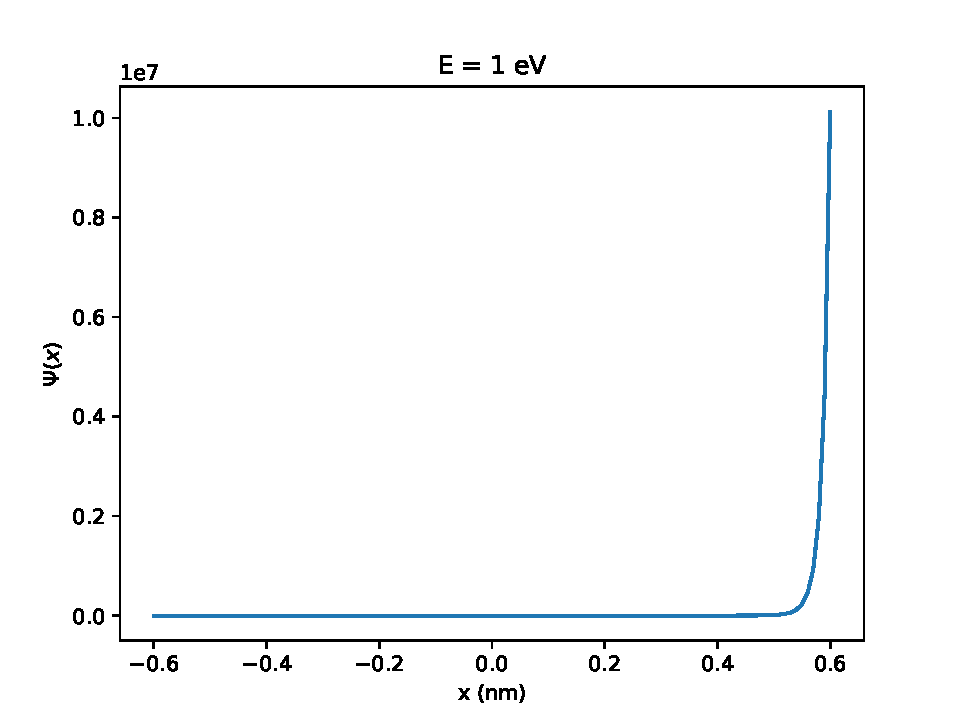
\includegraphics[width=.45\textwidth]{../figs/q1_linscale.pdf}
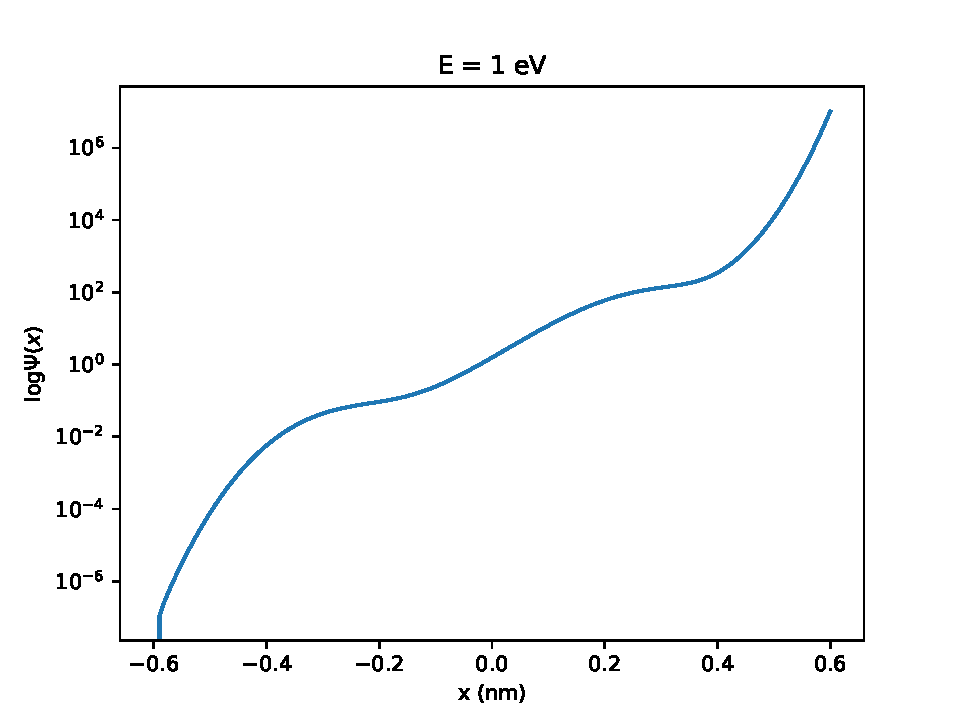
\includegraphics[width=.45\textwidth]{../figs/q1_logscale.pdf}
\end{center}
\captionof{figure}{Plot of $\Psi(x)$ fo 1 eV. On the left, we have a linear scale while, on the right, we have a logarithmic scale. Based on these, we can see that, even though the dramatic  increase exists, especially for the higher $x$, we can see that the exponential trend also exists in the lower $x$.}
\vspace{2em}
\noindent \normalsize{We would expect, if the 1eV was an energy eigenstate, our solution would not blow up since the \textit{nonphysical} increasing component of the solution would have had a coefficient of zero, leading to only a decreasing component to be the only contributing part. If we were propagating in a classically allowed region, even if we did not have a correct energy eigenstate and our \textit{nonphysical} increasing component had a non-zero contribution at the start, that contribution would have quickly died down.}
\\ \\
\noindent \normalsize{However, in this case, 1eV is not a correct energy eigenstate nor does it ever enter a classically allowed region (all level under $\sim 20$ eV is not classically allowed). In this case, our \textit{nonphysical} increasing component of our solution has a non-zero coefficient that stays fully as we propagate in our domain. This leads to the increasing component quickly dominating the solution leading to a ``blow up'' as $x$ increases.}
\\ \\
\noindent \Large{Question 2}
\\ \\
\normalsize{For even states, $\Psi'(0)=0$ since it should be an inflection point. As for odd states, $\Psi(0)=0$ since we should expect a parity shift at the origin.}
\newpage
\noindent \Large{Question 3}
\\ \\
\normalsize{The 6 lowest energy eigenvalues are: 5.8533 eV, 5.8896 eV, 15.3591 eV, 16.6689 eV, 22.5864 eV, and 27.6564 eV.}
\\ \\
\noindent \Large{Question 4}
\\ \\
\begin{center}
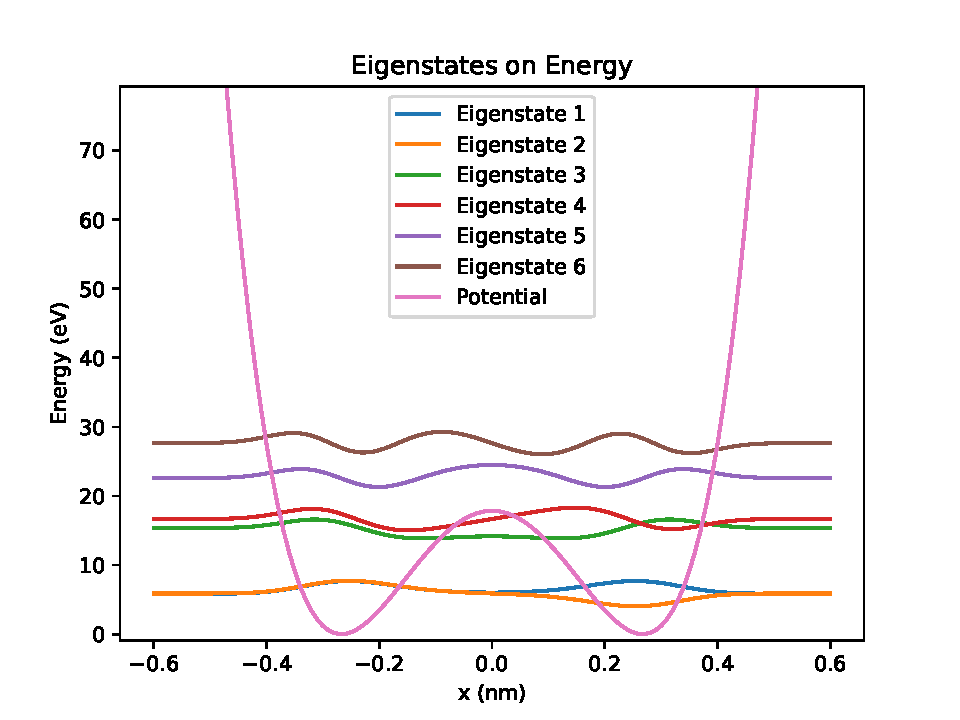
\includegraphics[width=.8\textwidth]{../figs/q4_eigenstates.pdf}
\end{center}
\vspace{2em}
\noindent \normalsize{The first thing that we can note is that even and odd states alternate as solutions, and that the spacings for the eigenstates are increasing. As for the two lowest eigenstates, we can see that they have a double anharmonic potential well, and as such, have a classically' forbidden region in between two classically allowed regions. This, however, is rectified by quantum mechanics with the help of quantum tunneling. They are also paired.}
\end{document}
